\begin{center}SPHERICAL HARMONICS.\end{center}
\begin{center}[1.]\end{center}
The following procedure decomposes $P$, \textit{a homogeneous function} of $x,y,z$ of order $i$, into \textit{pure spherical harmonics}.

Set
\[
\frac{\mathrm d\mathrm dP}{\mathrm dx^2}+\frac{\mathrm d\mathrm dP}{\mathrm dy^2}+\frac{\mathrm d\mathrm dP}{\mathrm dz^2}=P'=fP,\quad fP'=P'',\quad fP''=fP''',\ \text{etc.}
\]
and write $xx+yy+zz=\rho$ for brevity. One then puts $P$ in the form
\[
P=A+\rho B+\rho\rho C+\rho^3D+\text{and so on}
\]
with $A$, $B$, $C$, $D$, etc., as pure spherical harmonics. The following equations give this form
\SourceLeaf{637}
\[
\begin{aligned}
P&=A+\rho B+\rho\rho C+\rho^3D+\rho^4E+\text{and so on}\\
P'&=2(2i-1)B+4(2i-3)\rho C+6(2i-5)\rho\rho D\\
&\qquad+8(2i-7)\rho^3E+\text{and so on}\\
P''&=2.4(2i-3)(2i-5)C+4.6(2i-5)(2i-7)\rho D\\
&\qquad+6.8(2i-7)(2i-9)\rho\rho E+\text{and so on}\\
P'''&=2.4.6(2i-5)(2i-7)(2i-9)D\\
&\qquad+4.6.8(2i-7)(2i-9)(2i-11)\rho E+\text{and so on}\\
P''''&=2.4.6.8(2i-7)(2i-9)(2i-11)(2i-13)E+\text{and so on}
\end{aligned}
\]

One can also represent these equations by making the replacement indicated by $\rho\, .\, .\, .\,RR$ and treating only $R$ as variable in the differentiations.
\[
\frac{\mathrm d\mathrm d.R^{-i}P}{\mathrm dR^2}+R^{-i}.P'=i(i+1).R^{-i-2}P
\]

\begin{center}[2.]\\\textit{Geometric meaning of the spherical harmonics.}\end{center}
$P$ is the variable point.

$A$, $B$, $C$, $D$, etc., are fixed points.

First-order spherical harmonic $\alpha\cos PA$

Second order
\[
\alpha\cos PA.\cos PC+\beta\cos PB.\cos PD
\]
where $A$, $B$, $C$, $D$ refer to four faces of a regular octahedron.
\begin{center}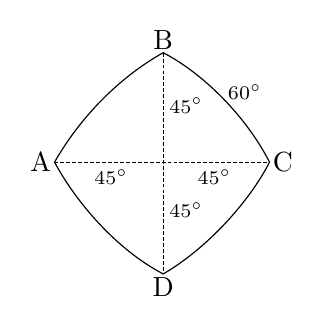
\begin{tikzpicture}[x=1cm,y=1cm,line width=.42pt,inner sep=1pt]
  \coordinate (A) at (-1.38,0);
  \coordinate (B) at (0,1.39);
  \coordinate (C) at (1.35,0);
  \coordinate (D) at (0,-1.42);
  \draw (A) .. controls (-1.06,.56) and (-.57,1.07) .. (B)
            .. controls (.52,1.12) and (1.06,.57) .. (C)
            .. controls (1.09,-.51) and (.55,-1.10) .. (D)
            .. controls (-.59,-1.11) and (-1.10,-.52) .. (A) -- cycle;
  \draw[dash pattern=on 1.4pt off .75pt] (A) -- (C) (B) -- (D);
  \node[left]  at (A) {$\mathrm A$};
  \node[above] at (B) {$\mathrm B$};
  \node[right] at (C) {$\mathrm C$};
  \node[below] at (D) {$\mathrm D$};
  \node[anchor=west]  at (.035,.72)  {\scriptsize $45^\circ$};
  \node[anchor=west]  at (.035,-.61) {\scriptsize $45^\circ$};
  \node[anchor=north] at (-.66,-.05) {\scriptsize $45^\circ$};
  \node[anchor=north] at (.65,-.05)  {\scriptsize $45^\circ$};
  \node[anchor=west]  at (.78,.89)   {\scriptsize $60^\circ$};
\end{tikzpicture}
\end{center}
Third order
\[
\alpha\cos PA.\cos PB.\cos PC+\beta\cos PA'.\cos PB'.\cos PC'
\]
where $A$, $B$, $C$ lie on one great circle and $A'$, $B'$, $C'$ on another, so that $AB=BC=CA=A'B'=B'C'=C'A'=120^0$ and the two circles intersect at right angles.

Fourth order. A sum of three products, each of four cosines. The three great circles intersect at right angles.

Fifth order. A sum of three products, each of five cosines. The three great circles intersect in a single point.

